Za stvaranje Linux-a bilo je potrebno nekoliko komponenti, najvažnija od kojih je Unix. Unix su stvorili Ken Tompson i Denis Riči. Njih dvojica, zajedno sa timom inžinjera u Belovim laboratorijama, su radili na Multics sistemu (\textbf{M}ultiplexed \textbf{I}nformation and \textbf{C}omputing \textbf{S}ervice), pravljen sa idejom da bude sistem koji može da radi više poslova u isto vreme. Tompson i Riči su u  tom periodu počeli da rade na svom sopstvenom sistemu, zasnovan na Multics-u, po imenu Unix, prvi put objavljen 1970. godine. Kasnije, kad je C programski jezik, koji je Riči napisao zajedno sa Brijanom Kernigenom, postao dovoljno razvijen, Unix je potpuno prepisan u C-u, što je pomoglo njegovom rasprostranjenju u razne akademske institucije i poslove. Zbog promenljive i prilagodljive prirode Unix-a, razni univerziteti su počeli da prave svoje verzije Unix-a, jedan od najpopularnijih je bio BSD (\textbf{B}erkeley \textbf{S}oftware \textbf{D}istribution), koji je još u upotrebi danas.\\

1983. godine, Ričard Stalman je započeo GNU projekat, namenjen da bude slobodna alternativa za Unix\cite{gnu}. Do ranih 90-ih, napisano je dovoljno softvera da se napravi citav operativni sistem. Jedino što je nedostajalo je "kernel" ili "jezgro" operativnog sistema, deo koji bi trebao sve ostale komponente da spoji. GNU je imao, i još ima, u pravljenu svoje kernel, GNU Hurd, ali nikad nije završen. Postojao je i kernel zasnovan na BSD-u, ali bez dovoljno funkcionalnosti.\\

Nedostatak besplatnog i korisnog kernel-a, je nerviralo Linusa Torvaldsa, pa je stoga odlučio da napiše svoji sopstveni. Torvalds je bio upoznat već sa Minix-om i sa GNU alatkama i dok je bio student informatike na Univerzitetu u Finskoj je počeo da radi na projektu koji bi kasnije postao Linux kernel. 25.-og avgusta 1991. godine, Torvalds je postavio na "Usenet newsgroup-i" o svom projektu. Nastavio je da bude projekat na kome je samo on radio, ali s vremenom je steklo sve više pažnje od drugih programera. Danas je preko 15000 programera \cite{linuxfoundation} doprinelo preko 17 miliona linija koda.\\
\begin{figure}[h]
\centering
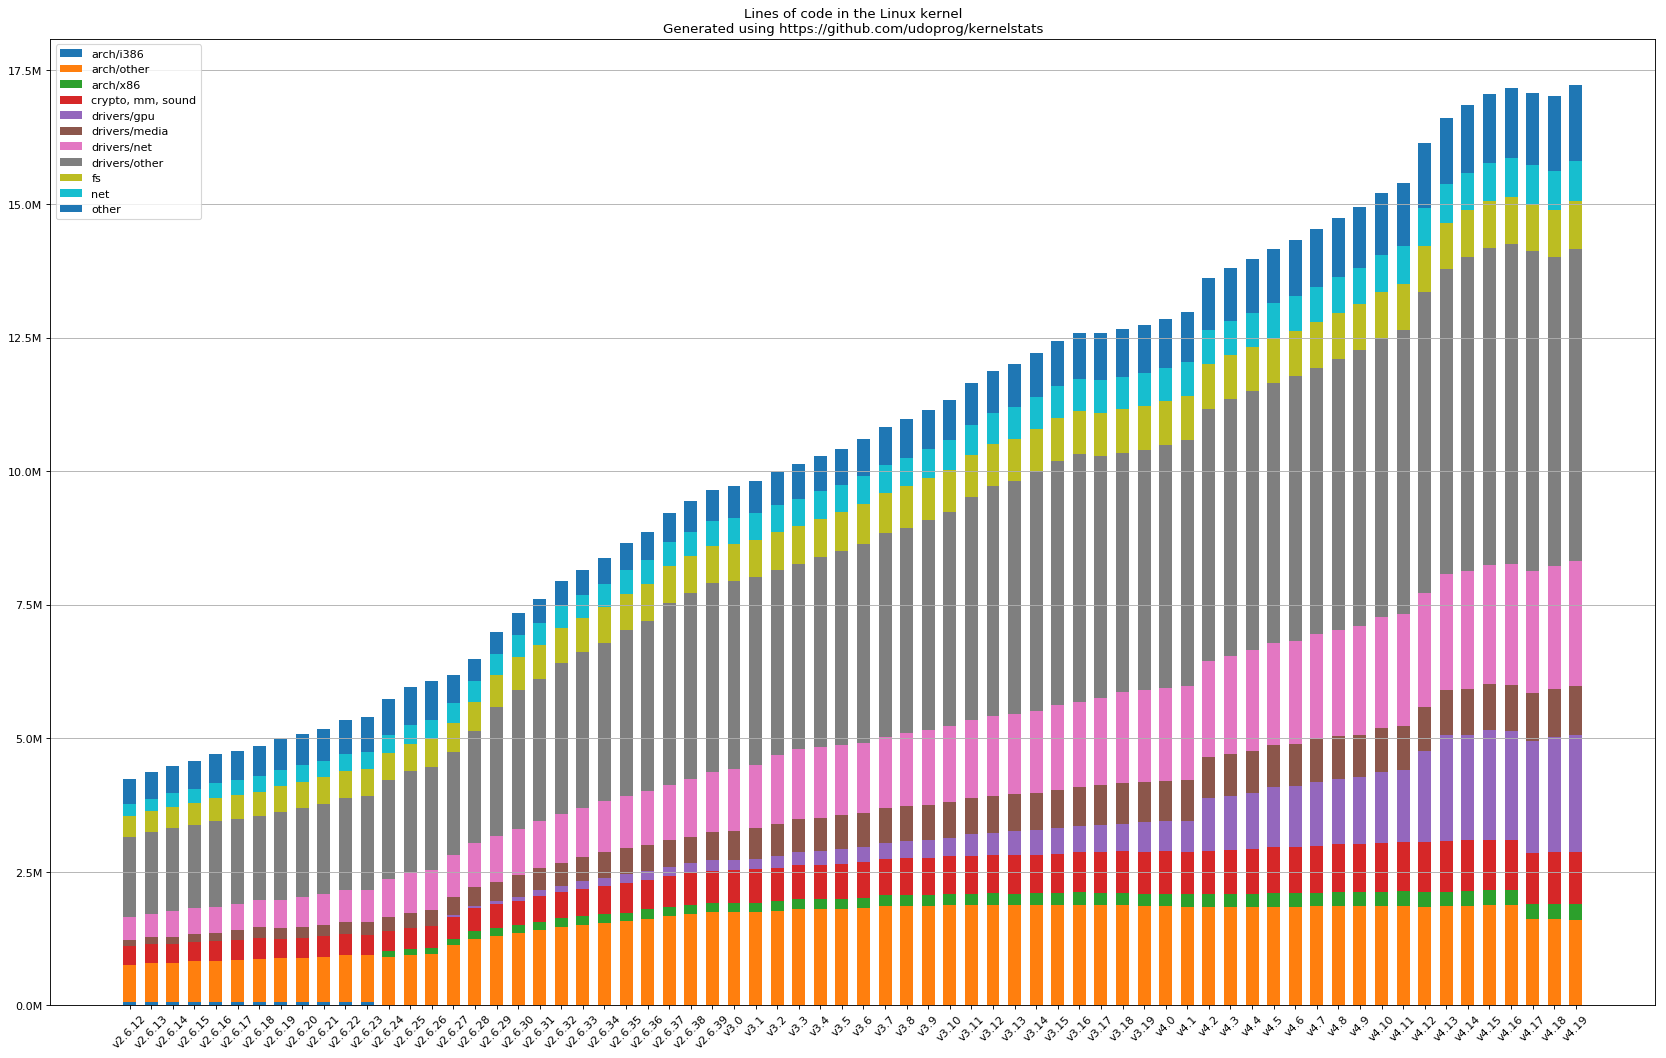
\includegraphics[scale=0.23]{loc}
\caption{Linija koda napisano od verzije 2.6.12 u milionima}
\end{figure}
